\begin{refsection}
\chapter{Appendix A} % Main chapter title
\label{appendix_A}

\section*{Energy gains during the experiment}

To evaluate the energy gains of \textit{Bombus} individuals during the experiments, we first determined the maximum energy gains per floral visits (Table \ref{tab:energy}). Then, we fit a model to predict the energy gains per visit for species $i$, using flower types as predictors:
\begin{equation}
	\kappa_{i} = \epsilon_{p}F_{pink}+\epsilon_{b}F_{blue} + \epsilon_{w}F_{white} + \epsilon_{y} F_{yellow} \,,
	\label{energy}
\end{equation}
where $\kappa_{i}$ is energy consumed per visit for species \textit{i}, $\epsilon_j$, are parameters that describe the energy gains, and $F_j$ are dummy variables that represent the type of flower visited. The subscripts denote the type of flowers by colors. We fit the model from Eq.~\ref{energy} to the data of energy per visit described in the main text. We fit this model using a Bayesian framework with Hamiltonian Monte Carlo (HMC) methods:

\begin{eqnarray}
  e_{i} &\sim& {\textrm {Normal}}(\mu_{i}, \sigma) \\
 \mu_{i} &=& \epsilon_{p}F_{pink} +\epsilon_{b}F_{blue} + \epsilon_{w}F_{white} + \epsilon_{y} F_{yellow} \\
{\epsilon_{p},\epsilon_{b}, \epsilon_{w}, \epsilon_{y}} &\sim& {\textrm {Normal}}(0,10) \\
\sigma &\sim& {\textrm {Student-t}} (3,0,10)
 \end{eqnarray}

 We ran four chains with a warmup of 1000 iterations and 1000 sampling iterations and using weakly informative priors. We fit our model and determined convergence using the same approach as described in \autoref{Bee_foraging}. Finally we used Bayes $R^{2}$ to estimate the proportion of variance explained by our model for new data.

 The model of energy consumption with flower types as predictors had a value of Bayes $R^{2}$ of 0.847. That is, if we were to fit the energy model to new data, we would expect it to estimate around 85\% of the variance. Furthermore, the parameter distribution of the energy mode yields estimates very similar to the maximum energy gains per visit Fig.~\ref{fig:flower_type}. That is, each time a bee visited a flower, we would expect it to gain as much energy as the maximum a flower has to offer. Thus, the more visits an individual makes, the more energy gains it obtains.

 \begin{table}[H]
 \centering
 \caption[Maximum energy gains per visit]{Maximum energy gains per visit, for each of the different flower types. Each visit triggered the automatic reward of of  10 $\mu$l, and each gram of sugar has 17 kilojoules of energy.}
 \label{tab:energy}
 \begin{tabular}{lcc}
 \toprule
 Flower type & Sucrose concentration & Max.\ kilojoules per visit \\ \midrule
 Blue        & 2.0 M                   & 0.1165                   \\
 White       & 1.5 M                 & 0.0877                   \\
 Yellow      & 1.0 M                   & 0.0581                   \\
 Pink        & 0.5 M                 & 0.0290                   \\ \bottomrule
 \end{tabular}
 \end{table}

 Indeed, plots of total number of floral visits per bee per trial and total energy gains per trial (Fig.~\ref{fig:energy_visits}) , show that energy gains are strongly correlated with the number of floral visits an individual makes. Thus, we can be confident that \textit{Bombus} individuals were consuming close to the full reward each time they visited an artificial flower.


 \begin{figure}[H]
     \centerline{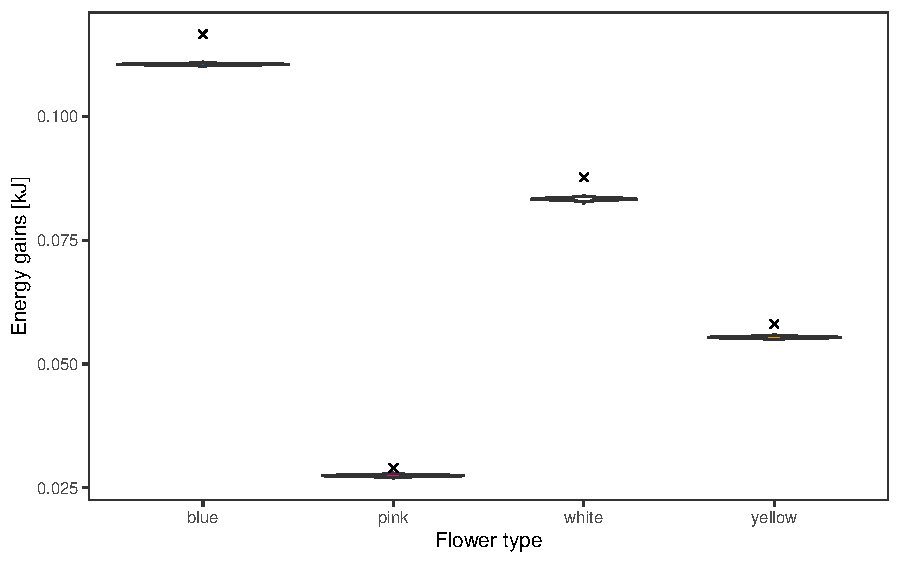
\includegraphics[width=0.9\textwidth]{figures/appendixA_fig1.pdf}}
     \caption[Posterior distribution of $\epsilon$ parameters from Eq.~\ref{energy}]{ Posterior distribution of $\epsilon$ parameters from Eq.~\ref{energy}. Each parameter estimates the mean energetic gain per visit (in kilojoules), per flower type. We have also indicated the maximum gains per visit of the different flower types with an x.  }
     \label{fig:flower_type}
 \end{figure}{}


 \begin{figure}[H]
     \centerline{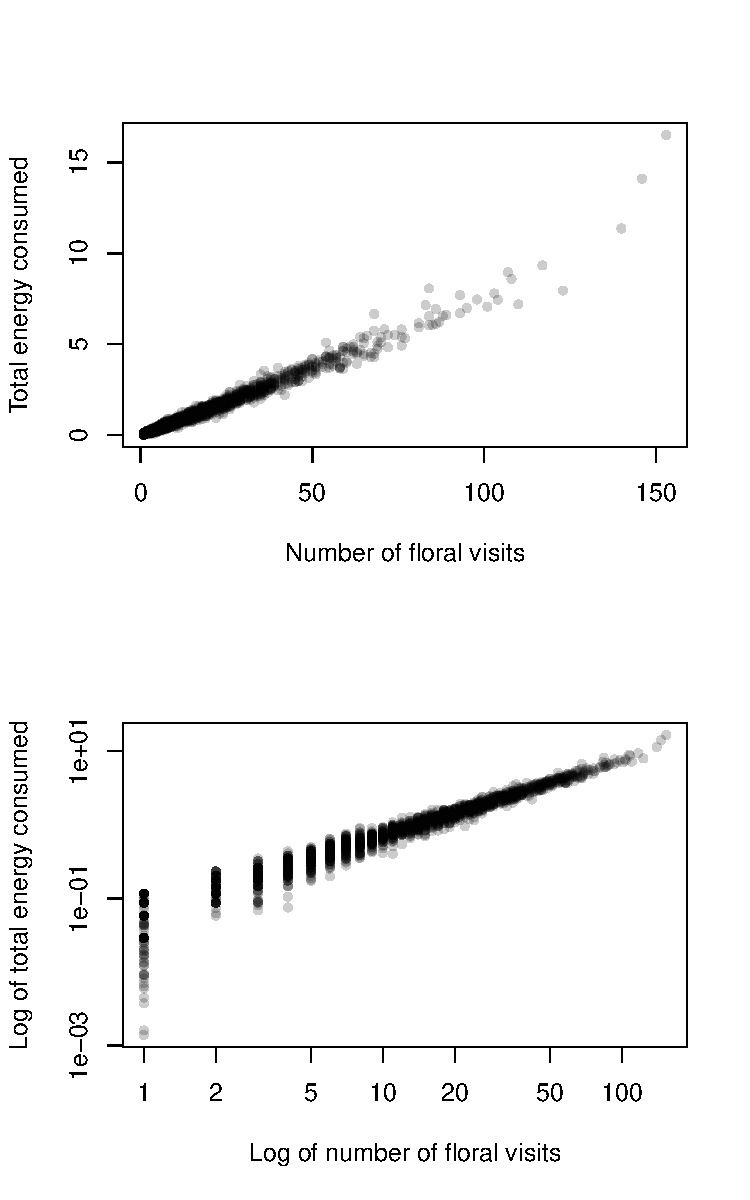
\includegraphics[height=0.7\textheight]{figures/appendixA_fig2.pdf}}
     \caption[Relationship between the total number of visits made by an individual bee and its total energy gains during an experiment trial.]{Relationship between the total number of visits made by an individual bee and its total energy gains during an experiment trial. In the top panel, the total energy consumed per trial is clearly an increasing function of the number of floral visits an individual makes during the trial. Each point corresponds to observations at the individual level. In the bottom panel, we show the same relationship with log-log axes. }
     \label{fig:energy_visits}
 \end{figure}{  }

\section*{Foraging trials and data structure}

In single-species trials, all but one of the factorial combinations of  conspecific co-foragers, pesticide exposure, and two levels of resource availability (instantaneous and delayed refill) had at least two replicates. The only exceptions were the combinations of  four and eight \textit{Bombus} individuals foraging under instantaneous floral refill and pesticide exposure. The third level of resource availability, intermediate floral refill time, was tested \textit{only} for 16 \textit{Bombus} individuals foraging at the same time, for the two levels of pesticide exposure (Table \ref{tab:si}).

In multi-species trials, all but two of the factorial combinations of bee species richness,  two levels of resource availability (instantaneous and delayed refill), and pesticide exposure had at least two replicates. The only exception was three foraging species with instantaneous refill and pesticide exposure. Furthermore, not all species of co-foragers were tested under all combinations of resource availability and pesticide exposure, making it impossible to fully disentangle their statistical interaction (Table \ref{tab:mu}).

In total, we tracked the time between floral visits and energy consumed by 735 \textit{Bombus} individuals across 139 single-species trials and by 277 \textit{Bombus} individuals across 112 multi-species trials. We excluded from the analysis the data from bumblebees that were completely inactive within trials (i.e.\ that did not record a single visit during the 75 minutes), since they do not provide information regarding visitation frequency or energy obtained per visit. Of the data collected from the active bees, we also excluded the first and last record of time and nectar consumption for every individual bumblebee within a trial, unless that individual only made one visit. We excluded those data points since previous research indicates that these points are less informative about foraging behavior and generate skewed data \citep{edwards_revisiting_2007}. The number of observations we examined amounts to 33919 records of times between floral visits.

\begin{table}[H]
\centering
\caption[Single-species foraging trials]{Single-species foraging trials. We show the number of trials for different combinations of \textit{Bombus} abundance, pesticide exposure and refill time. Pesticide exposure is a binary variable that equals to one when all individuals in the trial were subject to a sub-lethal doses of pesticide. Refill time is the time (in seconds) after which an artificial flower could dispense a new sucrose reward after a previous visit. }
\label{tab:si}
\begin{tabular}{@{}llll@{}}
\toprule
\textit{Bombus} abundance & Pesticide exposure & Refill time & Number of trials \\ \midrule
4       & 0                  & 0           & 2                    \\
4       & 0                  & 540         & 10                   \\
4       & 1                  & 0           & 0                    \\
4       & 1                  & 540         & 13                   \\
8       & 0                  & 0           & 2                    \\
8       & 0                  & 540         & 10                   \\
8       & 1                  & 0           & 0                    \\
8       & 1                  & 540         & 13                   \\
16      & 0                  & 0           & 5                    \\
16      & 0                  & 120         & 34                   \\
16      & 0                  & 540         & 15                   \\
16      & 1                  & 0           & 5                    \\
16      & 1                  & 120         & 14                   \\
16      & 1                  & 540         & 16                   \\ \bottomrule
\end{tabular}
\end{table}


\begin{table}[H]
\centering
\caption[Multi-species foraging trials]{Multi-species foraging trials. We show the number of trials for different combinations of species richness, pesticide exposure and two levels of resource availability. We also show the number of individuals of each species used in each trial as well as the number of trials per combination. Pesticide exposure and refill time have the same interpretation as in the single-species trials.}
\label{tab:mu}
\resizebox{\textwidth}{!}{\begin{tabular}{@{}llllllll@{}}
\toprule
Richness & Pesticide exposure & Refill time & \textit{Bombus}
abundance & \textit{Apis} abundance & \textit{Osmia} abundance & \textit{Megachile}  abundance& Number of trials \\ \midrule
2        & 0                  & 0           & 8               & 0             & 8             & 0                  & 7                    \\
2        & 0                  & 0           & 8               & 0             & 0             & 8                  & 5                    \\
2        & 0                  & 0           & 8               & 8             & 0             & 0                  & 5                    \\
2        & 1                  & 0           & 8               & 0             & 8             & 0                  & 2                    \\
2        & 0                  & 540         & 8               & 0             & 8             & 0                  & 7                    \\
2        & 0                  & 540         & 8               & 0             & 0             & 8                  & 5                    \\
2        & 0                  & 540         & 8               & 8             & 0             & 0                  & 5                    \\
2        & 1                  & 540         & 8               & 0             & 8             & 0                  & 6                    \\
2        & 1                  & 540         & 8               & 0             & 0             & 8                  & 4                    \\
2        & 1                  & 540         & 8               & 8             & 0             & 0                  & 6                    \\
3        & 0                  & 0           & 5               & 5             & 6             & 0                  & 3                    \\
3        & 0                  & 0           & 6               & 5             & 5             & 0                  & 1                    \\
3        & 0                  & 0           & 5               & 6             & 5             & 0                  & 1                    \\
3        & 0                  & 0           & 5               & 0             & 6             & 5                  & 3                    \\
3        & 0                  & 0           & 6               & 0             & 5             & 5                  & 2                    \\
3        & 0                  & 0           & 6               & 5             & 0             & 5                  & 2                    \\
3        & 0                  & 0           & 5               & 5             & 0             & 6                  & 1                    \\
3        & 0                  & 540         & 6               & 5             & 5             & 0                  & 1                    \\
3        & 0                  & 540         & 5               & 5             & 6             & 0                  & 3                    \\
3        & 0                  & 540         & 5               & 6             & 5             & 0                  & 1                    \\
3        & 0                  & 540         & 5               & 0             & 6             & 5                  & 3                    \\
3        & 0                  & 540         & 6               & 0             & 5             & 5                  & 3                    \\
3        & 0                  & 540         & 6               & 5             & 0             & 5                  & 3                    \\
3        & 1                  & 540         & 6               & 5             & 5             & 0                  & 5                    \\
3        & 1                  & 540         & 5               & 5             & 6             & 0                  & 2                    \\
3        & 1                  & 540         & 6               & 0             & 5             & 5                  & 4                    \\
3        & 1                  & 540         & 5               & 0             & 6             & 5                  & 1                    \\
3        & 1                  & 540         & 6               & 5             & 0             & 5                  & 1                    \\
4        & 0                  & 0           & 4               & 4             & 4             & 4                  & 5                    \\
4        & 1                  & 0           & 4               & 4             & 4             & 4                  & 5                    \\
4        & 0                  & 540         & 4               & 4             & 4             & 4                  & 5                    \\
4        & 1                  & 540         & 4               & 4             & 4             & 4                  & 5                    \\ \bottomrule
\end{tabular}}
\end{table}

\section*{Statistical Analysis}

We used hierarchical models to fit the data to the models described in the main text (Eqs.~9-11) because we have multiple observations from the same \textit{Bombus} individuals and to allow each of these individuals to deviate from the parameter's grand mean. For example, predicted times between floral visits for an individual \textit{b} of species \textit{i} given by the \textit{interference} model would be:
\begin{equation}
    \rho_{i,b} = (\alpha + \Delta \alpha_{b}) +  (\beta_{i}+ \Delta\beta_{ib})  (P_{i}-1) +    \sum_{j} (\beta_{j}+ \Delta\beta_{jb})P_{j}
\end{equation}
The three deviations from the grand means ($\Delta\alpha_{b}$, $\Delta\beta_{ib}$, $\Delta\beta_{jb}$) capture the individual specific response and are incorporated in a comparable manner to how random effects are included in mixed-effects models. This way to parameterize our models allowed us to estimate how each individual responded to the treatments, helped to control for pseudo-replication across individual bees, and pooled information across individual bees to still inform the grand mean when sample size was low We show how we incorporated the random effects in each model in  Table \ref{tab:random}.


Across all models, we assumed that the times between floral visits followed an exponential distribution that has a rate parameter $\rho_{i,b}$. We also required  the density-independent rate of all models to be positive,as a ``negative'' time would be unfeasible as a baseline. Thus we constrained the density independent parameters to be positive. Consequently, we fit non-linear models using the exponential family and the ``identity'' link. Again, using the \textit{interference} model as an example, our Bayesian one-level hierarchical model of times between floral visits for an individual \textit{b} may be written as:
  \begin{eqnarray}
   t_{i,b} &\sim& {\textrm{Exponential}}(\rho_{i,b}) \\
  \rho_{b} &=& e^{(\alpha + \Delta \alpha_{b})} +  (\beta_{i}+ \Delta\beta_{ib})  (P_{i}-1) +    \sum_{j} (\beta_{j}+ \Delta\beta_{jb})P_{j} \\
{\alpha,\beta_{i},\beta_{j}} &\sim& {\textrm{Normal}}(0,10) \\
{\Delta\alpha_{b}, \Delta\beta_{ib},\Delta\beta_{jb}}  &\sim&{\textrm{Multivariate Normal}} (\sigma,\gamma) \\
\sigma &\sim& {\text{Student-t}} (3,0,70)\\
\gamma &\sim& {\textrm{LKJcorr}}(1)
  \end{eqnarray}


  	\begin{sidewaystable}
  	\centering
  	\caption[Statistical models fitted to the data]{Statistical models fitted to the data. Each model includes fixed and random effects that together determine the time between floral visits. The \textit{null} model assumes that neither co-foraging species nor environmental conditions change the times between floral visits. The \textit{interference} model allows the number of visits to change only due to the number of co-foraging bees (i.e.\ it treats interference as constant across environmental conditions). Finally, the \textit{treatments} model allows the environmental conditions to have an effect on both the density-independent and density-dependent parameters.}
  	\label{tab:random}
  	\begin{tabular*}{\textwidth}{l @{\extracolsep{\fill}} clll}
  	\toprule
  	Model         & Eqn. in main text    & Parameter class & Fixed effects    & Random effects  \\ \midrule
  	\textit{null} & \ref{null} & density-independent & $\alpha$ & $\Delta \alpha_{b}$ \\
  	%\textit{null} & 7       &  \begin{tabular}[c]{@{}l@{}} \\ density-independent
  	%                           \\\end{tabular}    & \begin{tabular}[c]{@{}l@{}} \\$\alpha $
  	%                           \\\end{tabular}       &  \begin{tabular}[c]{@{}l@{}} \\$\Delta \ 	alpha_{b}$ \end{tabular}    \\ \midrule
  	\midrule
  	\multirow{3}{*}{\textit{interference}} & \multirow{3}{*}{\ref{interference_3}} & density-independent & $\alpha$ & $\Delta \alpha_{b}$ \\
  	& & conspecific-dependent & $ \beta_{i}$ & $\Delta \beta_{ib}$ \\
  	& & heterospecific-dependent & $ \beta_{j}$ & $\Delta \beta_{jb}$ \\
  	\midrule


  	\multirow{3}{*}{\textit{treatments}} & \multirow{3}{*}{\ref{treatments}} & density-independent & $\alpha,\alpha_{r},\alpha_{e}$ & $\Delta \alpha_{b} , \Delta \alpha_{rb} , \Delta \alpha_{eb}$ \\
  	& & conspecific-dependent & $ \beta_{i} , \beta_{ir}, \beta_{ie}$ & $\Delta \beta_{ib}, \Delta \beta_{irb} , \Delta \beta_{ieb}$ \\
  	& & heterospecific-dependent & $ \beta_{j}, \beta_{jr} , \beta_{je}$ & $\Delta \beta_{jb},  \Delta \beta_{jrb} , \Delta\beta_{jeb}$ \\
   \bottomrule
  	\end{tabular*}
  \end{sidewaystable}



\end{refsection}
